\chapter{What Does It Take to Build a Performant Selective Classifier?}

\section{Broader Impact}
\label{sec:broader_impact}

This work introduces a decomposition of the selective-classification gap into measurable components—Bayes noise, approximation error, ranking error, statistical noise, and deployment slack—offering practical guidance for improving abstaining classifiers. By diagnosing which source dominates in a given setting, our method supports more targeted model design and evaluation.

\paragraph{Positive Implications.}
Our decomposition improves transparency and supports safer deployment in high-stakes domains by helping practitioners understand whether their model underperforms due to ranking, capacity, or robustness. Because each gap component is explicitly quantified, our approach can serve as a tool for model debugging, monitoring, and fairer benchmarking.

\paragraph{Potential Risks.}
Selective classifiers may disproportionately defer on certain groups, amplifying disparities—a risk previously observed by~\citet{jones2020selective}. Additionally, institutions may exploit uncertainty estimates to justify \emph{strategic abstention}—deliberately deferring on individuals they prefer not to serve~\citep{rabanser2025confidential}. While our framework identifies which part of the gap drives poor performance, it does not control how deferred inputs are handled.

\paragraph{Mitigations.}
We recommend reporting gap components disaggregated by sensitive attributes, auditing scoring functions for spurious correlations, and documenting fallback policies. These steps are essential to ensure that abstention mechanisms improve reliability without undermining fairness.

\paragraph{Outlook.}
We hope this work encourages more precise evaluations of selective classifiers, shifting focus from aggregate calibration to interpretable, component-wise gap analysis that can inform both technical improvements and policy safeguards.


\section{Methods Extension}
\label{sec:meth_ext}

\subsection{Detailed Proof of Theorem~\ref{thm:gap}}
\label{app:proof-gap-ranking}

We restate the theorem for convenience.

\begin{theorem}[Selective classification gap; detailed]
Fix a coverage level \(c\in(0,1]\), a score function \(g(\cdot,h)\),
and its associated population threshold
\(t_c\) satisfying \(\Pr\bigl(g(X,h)\ge t_c\bigr)=c\).
Define the accepted region \(A_c:=\{x:g(x,h)\ge t_c\}\) and
the oracle region
\(A_c^{\star}:=\{x:\eta_h(x)\text{ is among the largest }c\text{-fraction}\}\).
With the error terms
\begin{align}
\varepsilon_{\mathrm{Bayes}}(c)
&= \mathbb{E}\left[1 - \max\{\eta(X), 1 - \eta(X)\} \mid X \in A_c \right], \\
\varepsilon_{\mathrm{approx}}(c)
&= \mathbb{E}\left[ \lvert \eta_h(X) - \eta(X) \rvert \mid X \in A_c \right], \\
\varepsilon_{\mathrm{rank}}(c)
&= \mathbb{E}\left[ \eta_h(X) \mid X \in A_c^{\star} \right]
 - \mathbb{E}\left[ \eta_h(X) \mid X \in A_c \right] \;\;(\ge 0),
\end{align}
the population gap satisfies
\begin{equation}
\label{eq:pop-gap-app}
\Delta(c)=\overline{\operatorname{acc}}\bigl(a_{\mathrm{full}},c\bigr)
-\operatorname{acc}_c(h,g)
\;\le\;
\varepsilon_{\mathrm{Bayes}}(c)
+\varepsilon_{\mathrm{approx}}(c)
+\varepsilon_{\mathrm{rank}}(c).
\end{equation}
Moreover, let \(\widehat{\Delta}(c)\) be the empirical gap computed on
\(n\) independent test samples.  Then for any
\(\delta\in(0,1)\), with probability at least \(1-\delta\),
\begin{equation}
\label{eq:emp-gap-app}
\widehat{\Delta}(c)
\;\le\;
\varepsilon_{\mathrm{Bayes}}(c)
+\varepsilon_{\mathrm{approx}}(c)
+\varepsilon_{\mathrm{rank}}(c)
+ C\sqrt{\frac{\log(1/\delta)}{n}},
\end{equation}
where \(C>0\) is an absolute constant.
\end{theorem}

\begin{proof}
We split the argument into four self‑contained steps.

\textbf{Step 0.  Oracle upper bound revisited.}
For completeness we justify the piecewise form of
\(\overline{\operatorname{acc}}\bigl(a_{\mathrm{full}},c\bigr)\)
in Definition~\ref{def:poub}.
Because
\(a_{\mathrm{full}}=\Pr(h(X)=Y)=\mathbb E[\eta_h(X)]\),
the set
\(\{x:\eta_h(x)=1\}\) has probability mass at least
\(a_{\mathrm{full}}\).  Hence an oracle that retains the
highest‑confidence points achieves perfect accuracy for all
coverages \(c\le a_{\mathrm{full}}\).  For \(c>a_{\mathrm{full}}\),
the best it can do is include \emph{only} those perfect points
plus a \((c-a_{\mathrm{full}})\)-fraction of the remaining
examples, which contribute at worst zero accuracy.  Therefore
\begin{equation}
\overline{\operatorname{acc}}(a_{\mathrm{full}},c)=
\frac{a_{\mathrm{full}}}{c},
\qquad
a_{\mathrm{full}}<c<1.
\end{equation}

\textbf{Step 1.  Algebraic decomposition of the gap.}
Recall that
\(\operatorname{acc}_c(h,g)
   =\mathbb E[\eta_h(X)\mid X\in A_c]\).
We repeatedly add and subtract the same quantity:
\begin{align}
\Delta(c)
&:=\overline{\operatorname{acc}}(a_{\mathrm{full}},c)
  -\operatorname{acc}_c(h,g)  \notag\\[2pt]
&=\overline{\operatorname{acc}}(a_{\mathrm{full}},c)
  -\mathbb E[\eta_h\mid A_c^{\star}]
  \;+\;\mathbb E[\eta_h\mid A_c^{\star}]
  -\mathbb E[\eta_h\mid A_c] \notag\\
&\le
  \mathbb E[\eta_h\mid A_c^{\star}]
  -\mathbb E[\eta_h\mid A_c]                   \tag{rank}\\
&\quad
  +\,\mathbb E[\eta_h-\mathbb{I}_{\{h=Y\}}\mid A_c] \tag{approx+Bayes}\\
&= \varepsilon_{\mathrm{rank}}(c)
   +\varepsilon_{\mathrm{approx}}(c)
   +\varepsilon_{\mathrm{Bayes}}(c).
\end{align}
\textbf{Explanation of the two labelled inequalities.}
\begin{enumerate}
    \item \textbf{(rank)} isolates the ranking error, $\varepsilon_{\text{rank}}(c) := \mathbb{E}[\eta_h \mid A_c^{\star}] - \mathbb{E}[\eta_h \mid A_c]$.  The inequality holds because the remaining term from the previous line, $\overline{\operatorname{acc}}(a_{\text{full}}, c) - \mathbb{E}[\eta_h \mid A_c^{\star}]$, is a non-negative quantity that is bounded by the error sources introduced in the next step.
   \item \textbf{(approx+Bayes)} adds and subtracts \(\eta(X)\) inside the
   expectation, then splits the absolute value:
   \begin{equation}
   \eta_h-I_{\{h=Y\}}
   =(\eta_h-\eta)+(\eta-I_{\{h=Y\}}).
   \end{equation}
   The second summand satisfies the deterministic bound
   \(
     |\eta(X)-I_{\{h=Y\}}|
     = \max\{\eta,1-\eta\}-I_{\{h=Y\}}
     \le 1-\max\{\eta,1-\eta\},
   \)
   yielding exactly \(\varepsilon_{\mathrm{Bayes}}(c)\).
   The first summand contributes
   \(\varepsilon_{\mathrm{approx}}(c)\).
\end{enumerate}

\textbf{Step 2.  Non‑negativity of \(\varepsilon_{\mathrm{rank}}(c)\).}
Because \(\eta_h(X)\in[0,1]\) and
\(A_c^{\star}\) contains the \(c\)-fraction of points with the
largest \(\eta_h\)-values,
\(\mathbb E[\eta_h\mid A_c^{\star}]
 \ge\mathbb E[\eta_h\mid A_c]\),
hence \(\varepsilon_{\mathrm{rank}}(c)\ge0\) as stated.

\textbf{Step 3.  Finite‑sample deviation.}
Let \(\widehat{\mu}\) be any empirical average of a
\([0,1]\)-valued random variable with expectation \(\mu\).
Hoeffding’s inequality gives
\(\Pr(\lvert\widehat{\mu}-\mu\rvert>\epsilon)
   \le 2e^{-2n\epsilon^2}\).
Apply this bound separately to the three empirical estimates that
constitute \(\widehat{\Delta}(c)\), and take a union bound with
\(\epsilon=\sqrt{\tfrac{\log(6/\delta)}{2n}}\).
This yields, with probability at least \(1-\delta\),
\(
  \lvert\widehat{\Delta}(c)-\Delta(c)\rvert
  \le C\sqrt{\log(1/\delta)/n}
\)
for an absolute constant \(C\).
Combining with \eqref{eq:pop-gap-app} proves
\eqref{eq:emp-gap-app}.

\textbf{Step 4.  Connection to ranking distance.}
Define the mass of mis‑ordered points
\(D_{\mathrm{rank}}(c):=
 \Pr\bigl(X\in A_c^{\star}\setminus A_c\bigr)
 +\Pr\bigl(X\in A_c\setminus A_c^{\star}\bigr)\).
Because \(\eta_h\in[0,1]\),
\begin{align}
\varepsilon_{\mathrm{rank}}(c)
&=\mathbb E[\eta_h\mid A_c^{\star}]
  -\mathbb E[\eta_h\mid A_c]   \\[2pt]
&\le\bigl\|\eta_h\bigr\|_{\infty}\,
       D_{\mathrm{rank}}(c)        \\[2pt]
&\le D_{\mathrm{rank}}(c).
\end{align}
Hence \(\varepsilon_{\mathrm{rank}}(c)=0\)
if and only if \(A_c=A_c^{\star}\).

\smallskip\noindent
This completes the proof.
\end{proof}

\paragraph{Multiclass Remark.}
For \(K>2\) labels, define
\(\eta(x)=\bigl(\Pr(Y=1\mid x),\dots,\Pr(Y=K\mid x)\bigr)\)
and its complement confidence
\(\eta^{\max}(x)=\max_{k}\eta_k(x)\).
Then the inequality
\(\lvert\eta^{\max}-I_{\{h=Y\}}\rvert
 \le 1-\eta^{\max}\)
replaces the binary bound above, and the rest of the argument
goes through verbatim.  The approximation term becomes
\(\mathbb E[\lVert\eta_h-\eta\rVert_1\mid A_c]\);
all other quantities are unchanged.


\subsection{When Can Temperature Scaling Re-rank Confidence Scores?}
\label{app:ts-rerank}

Temperature scaling multiplies every logit by the same factor
$1/T\;(T>0)$ before the softmax,
\begin{equation}
p^{(T)}_j(x)= \frac{\exp(z_j(x)/T)}{\sum_k \exp(z_k(x)/T)}.
\end{equation}
Although the predicted label $\arg\max_j z_j(x)$ is invariant to~$T$,
the \emph{confidence score}
$s_T(x)=\max_j p^{(T)}_j(x)$
can change its \emph{cross-sample} ordering.

\paragraph{General form.}
Let $j_\star=\arg\max_j z_j(x)$ and
$r_j(x)=\exp\bigl(z_j(x)-z_{j_\star}(x)\bigr)\;(j\ne j_\star)$.
Then
\begin{equation}
  s_T(x)=\frac{1}{1+\sum_{j\ne j_\star} r_j(x)^{1/T}}.
  \label{eq:st-general}
\end{equation}
For binary classification, the sum has a single term and
\eqref{eq:st-general} collapses to the familiar logistic form
$s_T(x)=1/(1+e^{-\Delta/T})$ with
$\Delta=z_{j_\star}-z_{3-j_\star}$.

\paragraph{Two-sample condition.}
For two inputs $x_1,x_2$ let
$S_i(T)=\sum_{j\ne j_\star^{(i)}}r_{ij}^{1/T}$.
Because each $r_{ij}\le 1$, every $r_{ij}^{1/T}$ is monotone non-decreasing in $T$ (strictly increasing unless there is a tie),
and the ordering $s_T(x_1)>s_T(x_2)$ can change
exactly at those temperatures $T$ where $S_1(T) = S_2(T)$.

\paragraph{Illustrative example ($K=3$).}
\begin{equation}
z^{(1)}=(-2,-3,-3),\quad z^{(2)}=(0,-0.1,-3).
\end{equation}
At $T=1$ one finds
$s_1(x_1)=0.576>0.512=s_1(x_2)$,
while at $T=3$ we see that
$s_3(x_1)=0.411<0.428=s_3(x_2)$,
so temperature scaling would now accept $x_2$ before $x_1$.

\paragraph{How likely is a swap?}
Equation~\eqref{eq:st-general} shows that a swap requires the
one-dimensional curves $S_1(T)$ and $S_2(T)$ to intersect.  Since the
curves are continuous and monotone, the intersection occurs—
if at all—at isolated temperatures and only when the competing logit
patterns are finely tuned.

\paragraph{Practical implication.}
Temperature scaling can \emph{in principle} tighten the
selective-classification gap, but only for the vanishingly small subset
of inputs whose non-maximum logits happen to satisfy
$S_1(T^\star)=S_2(T^\star)$.  To obtain a meaningful re-ordering one
must therefore adopt \emph{non-monotone} calibration strategies.


\subsection{Additional Contingent Slack}
\label{app:extra-slack-omitted}

In the main text (Sec.~\ref{sec:extra-slack-short}) we folded all implementation‐level imperfections into a single residual term \(\varepsilon_{\text{misc}}(c)\), retaining only optimization error and distribution shift explicitly. Here we list two further slack terms omitted there:

\begin{enumerate}[leftmargin=1.2em]
  \setcounter{enumi}{2}
  \item \textbf{Threshold‐selection noise \(\varepsilon_{\text{thr}}(c)\).}\\
    When the coverage threshold \(\hat t_c\) is chosen on a validation set of size \(m\), the realized coverage deviates from the target \(c\) by 
    \begin{equation}
      O\bigl(\sqrt{c(1-c)/m}\bigr),
    \end{equation}
    inducing a corresponding vertical shift in selective accuracy.

  \item \textbf{Tie‐breaking / score quantization \(\varepsilon_{\text{tie}}(c)\).}\\
    Discrete confidence values (e.g.\ low‐precision logits) create equivalence classes of samples with identical scores.  If \(\kappa\) denotes the maximum number of tied samples at any score level, then
    \begin{equation}
      \varepsilon_{\text{tie}}(c)
      \;\le\;
      \frac{\kappa}{n},
    \end{equation}
    where \(n\) is the size of the evaluation set.
\end{enumerate}

\noindent\textbf{Residual slack revisited.}  Together with optimization error \(\varepsilon_{\text{opt}}\) and shift \(\varepsilon_{\text{shift}}(c)\), these yield
\begin{equation}
  \varepsilon_{\text{misc}}(c)
  = \varepsilon_{\text{opt}}
  + \varepsilon_{\text{shift}}(c)
  + \varepsilon_{\text{thr}}(c)
  + \varepsilon_{\text{tie}}(c).
\end{equation}

\section{Practitioner Checklist for Tightening the Selective-Classification Gap}
\label{app:practical-checklist}

Below is an expanded, actionable checklist to help practitioners systematically tackle each component of the selective-classification gap.  For each item, we list concrete steps, recommended tools, and pointers to reduce the corresponding error term.

\begin{itemize}[leftmargin=1.5em]

  \item \textbf{\(\varepsilon_{\text{approx}}\) — Shrink Approximation Error}
    \begin{itemize}[leftmargin=1.25em]
      \item \emph{Model capacity:} increase depth/width (e.g.\ ResNet-50→ResNeXt), or use state-of-the-art architectures (Vision Transformers, ConvNeXt).
      \item \emph{Pre-training:} leverage self-supervised (SimCLR, BYOL) or foundation models (CLIP, DINO) for strong features.
      \item \emph{Distillation:} apply teacher–student fine-tuning (logit matching, hint layers).
      \item \emph{Data augmentation:} use AutoAugment, RandAugment or MixUp / CutMix to expose model to diverse examples.
    \end{itemize}

  \item \textbf{\(\varepsilon_{\text{rank}}\) — Improve Ranking Calibration:}
    \begin{itemize}[leftmargin=1.25em]
      \item \emph{Non-monotone recalibration:} try matrix scaling or vector/Dirichlet scaling.
      \item \emph{Feature-aware scoring:} train a small “confidence head” \(g_\psi(h(x), x)\) on held-out data to predict correctness.
      \item \emph{Conformal methods:} implement conformal p-value scoring (split conformal, Mondrian conformal) to adjust rankings.
      \item \emph{Binning approaches:} use Bayesian Binning into Quantiles (BBQ) or adaptive histogram binning with bin-wise re-ordering.
    \end{itemize}

  \item \textbf{\(\varepsilon_{\text{opt}}\) — Reduce Optimization Error:}
    \begin{itemize}[leftmargin=1.25em]
      \item \emph{Convergence diagnostics:} monitor training vs.\ validation loss; extend epochs until plateau.
      \item \emph{Learning-rate schedules:} employ cosine, OneCycle, or cyclical LR to escape local minima.
      \item \emph{Early stopping / checkpoints:} save and ensemble top-\(k\) checkpoints (e.g.\ last 5) to smooth out optimization noise.
      \item \emph{Regularization:} apply weight decay, dropout, or stochastic depth to improve generalization.
    \end{itemize}

  \item \textbf{\(\varepsilon_{\text{Bayes}}\) — Quantify Irreducible Noise:}
    \begin{itemize}[leftmargin=1.25em]
      \item \emph{Repeated labels:} collect multiple human annotations (e.g.\ CIFAR-10N) to estimate label disagreement.
      \item \emph{Noise-robust training:} use noise-aware losses (Bootstrapping, Taylor loss) when Bayes-noise is high.
      \item \emph{Dataset curation:} identify and remove or relabel ambiguous examples via active learning or consensus filtering.
    \end{itemize}

  \item \textbf{\(\varepsilon_{\text{stat}}\) — Control Statistical Slack:}
    \begin{itemize}[leftmargin=1.25em]
      \item \emph{Validation set size:} allocate a sufficiently large hold-out set (e.g.\ 10–20\% of the total data) for threshold estimation.
      \item \emph{Confidence intervals:} use distribution-free quantile bounds (e.g.\ DKW, Clopper–Pearson) to set conservative \(\tau_c\).
      \item \emph{Cross-validation:} average thresholds over \(k\) folds to reduce variance.
    \end{itemize}

  \item \textbf{\(\varepsilon_{\text{shift}}\) — Mitigate Distribution Shift:}
    \begin{itemize}[leftmargin=1.25em]
      \item \emph{Shift detection:} monitor covariate shifts via two-sample tests (MMD, KL divergence) between train/test features.
      \item \emph{Importance weighting:} re-weight training or calibration data by density ratio estimates (Kernel mean matching).
      \item \emph{Domain adaptation:} finetune on small in-domain samples, or use unsupervised adaptation (AdaBN, domain-Adversarial nets).
      \item \emph{Test-time adaptation:} apply batch-norm calibration or test-time training on incoming data.
    \end{itemize}

  \item \textbf{\(\varepsilon_{\text{thr}}\) — Threshold–Selection Noise:}
    \begin{itemize}[leftmargin=1.25em]
      \item \emph{Bootstrap resampling:} compute \(\tau_c\) over many resamples to estimate its standard error.
      \item \emph{Smooth thresholds:} interpolate between adjacent scores rather than snapping to the nearest observed value.
    \end{itemize}

  \item \textbf{\(\varepsilon_{\text{tie}}\) — Tie-Breaking \& Score Quantization:}
    \begin{itemize}[leftmargin=1.25em]
      \item \emph{Higher precision:} increase float precision (FP16→FP32→FP64) or logits bit-width.
      \item \emph{Dithering:} add small random noise to scores before thresholding to break ties.
    \end{itemize}

\end{itemize}

\noindent\textbf{Putting it all together.}  
After addressing each bullet above, recompute your selective accuracy–coverage curve and compare to the oracle bound (Def.~\ref{def:poub}).  Iterating over these steps will systematically shrink \(\widehat\Delta(c)\) toward its irreducible floor.


\section{Experimental Details}
\label{sec:exp_det}

\subsection{Computational Resources}
\label{app:comp_res}

Our experiments were conducted on a mix of GPU-equipped compute nodes with varying hardware configurations. Some machines are equipped with Intel Xeon Silver CPUs (10 cores, 20 threads) and 128GB of RAM, each hosting 4× NVIDIA GeForce RTX 2080 Ti GPUs with 11GB VRAM. Others feature AMD EPYC 7643 processors (48 cores, 96 threads), 512GB of RAM, and 4× NVIDIA A100 GPUs, each with 80GB VRAM.

\subsection{Hyper-Parameters}
\label{app:hyperparams}

We follow standard literature-recommended training settings across all datasets. For each architecture–dataset pair, we use a fixed learning rate, weight decay, and batch size as detailed below:

\begin{itemize}[leftmargin=1em]
    \item \textbf{SimpleCNN:}
    \begin{itemize}[leftmargin=1em]
        \item Learning rate: 0.01
        \item Weight decay: \(1\times10^{-4}\)
        \item Batch size: 128
    \end{itemize}

    \item \textbf{ResNet-18:}
    \begin{itemize}[leftmargin=1em]
        \item Learning rate: 0.1 for CIFAR datasets; 0.01 for Stanford Cars, Camelyon17
        \item Weight decay: \(5\times10^{-4}\)
        \item Batch size: 128
    \end{itemize}

    \item \textbf{WideResNet-50-2:}
    \begin{itemize}[leftmargin=1em]
        \item Same settings as ResNet-18
    \end{itemize}

    \item \textbf{Epochs:}
    \begin{itemize}[leftmargin=1em]
        \item 200 epochs for all datasets except Camelyon17, which uses 10
    \end{itemize}

    \item \textbf{Optimization:} SGD with momentum 0.9, Nesterov enabled, and a cosine annealing learning rate schedule.

    \item \textbf{Selective prediction methods:}
    \begin{itemize}[leftmargin=1em]
        \item \texttt{MSP}: Standard cross-entropy training
        \item \texttt{SAT}: Cross-entropy pretraining for half of training epochs, followed by Self-Adaptive Training (momentum \(0.9\)) with an extra abstain class
    \end{itemize}
\end{itemize}

All experiments use fixed random seeds for reproducibility and standard data augmentation per dataset (random crops, flips, normalization).


\subsection{SimpleCNN Architecture}
\label{app:simplecnn}

\noindent
The SimpleCNN model is a compact convolutional neural network used for experiments on lower-resolution image datasets. The architecture is defined by the following sequence of layers:
\begin{itemize}
  \item A $3 \times 3$ convolution with 32 filters and padding 1, followed by ReLU and $2 \times 2$ max-pooling.
  \item A second $3 \times 3$ convolution with 64 filters and padding 1, followed by ReLU and $2 \times 2$ max-pooling.
  \item A flattening layer, followed by a fully connected layer with 128 hidden units and ReLU activation.
  \item A final fully connected layer projecting to the number of output classes.
\end{itemize}

Let \( s = \texttt{input\_size} // 4 \) denote the spatial resolution after two $2\times2$ pooling layers. Then, the full model is:
\[
\begin{aligned}
\texttt{SimpleCNN}(x) =\;&
\texttt{Linear}\big(128 \to \texttt{num\_classes}\big) \circ \texttt{ReLU} \circ \\
&\texttt{Linear}\big(64 \cdot s^2 \to 128\big) \circ \texttt{Flatten} \circ \\
&\texttt{MaxPool2d} \circ \texttt{ReLU} \circ \texttt{Conv2d}(32 \to 64) \circ \\
&\texttt{MaxPool2d} \circ \texttt{ReLU} \circ \texttt{Conv2d}(3 \to 32)(x)
\end{aligned}
\]


\vspace{0.5em}
\noindent
The number of output classes is set as follows:
\[
\texttt{num\_classes} = 
\begin{cases}
10 & \text{for CIFAR-10}, \\
100 & \text{for CIFAR-100}, \\
196 & \text{for Stanford Cars}, \\
2 & \text{for Camelyon17}, \\
\end{cases}
\quad \text{with an optional extra class if \texttt{extra\_class} is True.}
\]

\vspace{0.5em}
\noindent
The input size is dataset-dependent and set to:
\[
\texttt{input\_size} = 
\begin{cases}
32 & \text{for CIFAR-10 and CIFAR-100}, \\
224 & \text{for Stanford Cars, Camelyon17}. 
\end{cases}
\]
The model structure is summarized below:
\begin{lstlisting}[language=Python]
SimpleCNN(
  (net): Sequential(
    (0): Conv2d(3, 32, kernel_size=(3, 3), stride=(1, 1), padding=1)
    (1): ReLU()
    (2): MaxPool2d(kernel_size=2, stride=2)
    (3): Conv2d(32, 64, kernel_size=(3, 3), stride=(1, 1), padding=1)
    (4): ReLU()
    (5): MaxPool2d(kernel_size=2, stride=2)
    (6): Flatten(start_dim=1)
    (7): Linear(in_features=4096, out_features=128)
    (8): ReLU()
    (9): Linear(in_features=128, out_features=num_classes)
  )
)
\end{lstlisting}


\subsection{Synthetic Distribution Shifts on Two Moons}
\label{app:twomoons-shifts}

To evaluate robustness under controlled covariate shifts, we apply a series of synthetic affine transformations to the test set of the standard two moons dataset. Each transformation simulates a distinct type of distribution shift:

\begin{itemize}
    \item \textbf{Original:} No transformation; the unperturbed test set.
    
    \item \textbf{Shear:} A shear transformation along the \(x\)-axis defined by:
    \begin{equation}
    \text{Shear matrix} \quad 
    S = \begin{bmatrix} 1 & 1.25 \\ 0 & 1 \end{bmatrix},
    \quad\text{so that} \quad 
    x' = Sx = 
    \begin{bmatrix}
    x + 1.25y \\
    y
    \end{bmatrix}.
    \end{equation}
    
    \item \textbf{Rotation:} A rotation by 30 degrees counterclockwise, using:
    \begin{equation}
    R = 
    \begin{bmatrix}
    \cos \theta & -\sin \theta \\
    \sin \theta & \cos \theta
    \end{bmatrix},
    \quad \theta = \frac{\pi}{6}.
    \end{equation}
    
    \item \textbf{Translation:} A shift of the input space by a fixed vector:
    \begin{equation}
    x' = x + t, \quad \text{where} \quad t = \begin{bmatrix} 1.0 \\ -0.5 \end{bmatrix}.
    \end{equation}
\end{itemize}

\noindent
Each transformation is applied to the test data matrix \( X_{\text{test}} \) via matrix multiplication or translation, yielding the following test sets:
\begin{equation}
\begin{aligned}
\text{Original:} &\quad X_{\text{test}} \\
\text{Shear:}    &\quad X_{\text{test}} \cdot S^\top \\
\text{Rotation:} &\quad X_{\text{test}} \cdot R^\top \\
\text{Translation:} &\quad X_{\text{test}} + t
\end{aligned}
\end{equation}

These transformations create meaningful distribution shifts while preserving label semantics, enabling precise evaluations of model robustness under shift.

\begin{figure}[t]
    \centering
    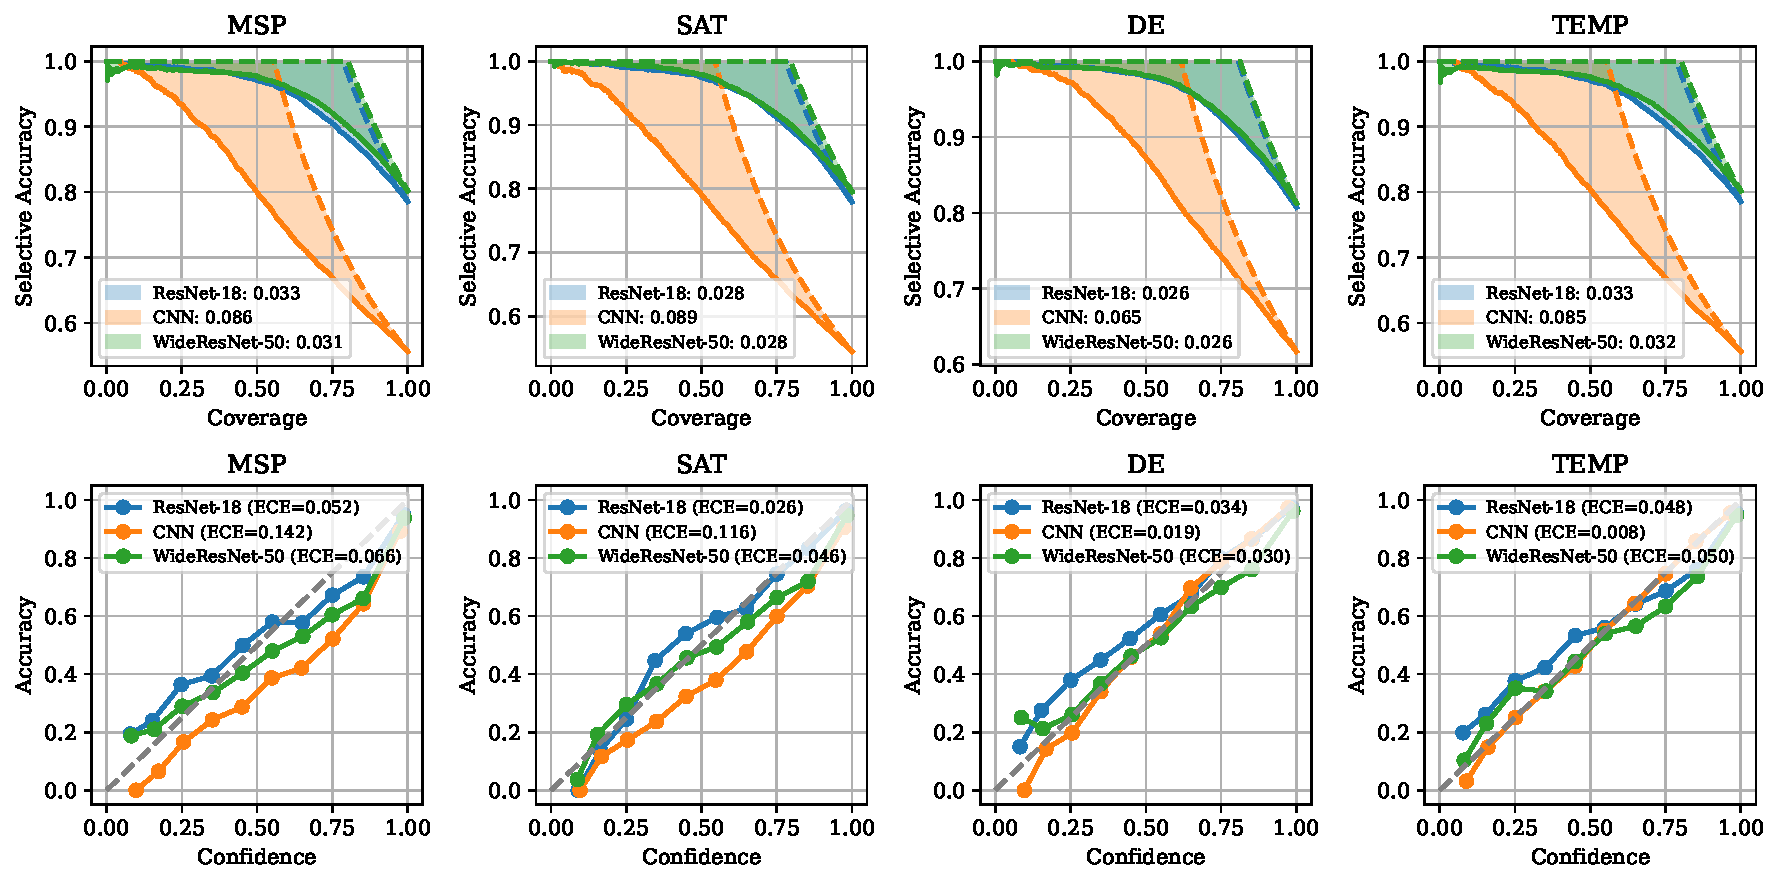
\includegraphics[width=1\linewidth]{figs/sc_bounds/cifar100_calibration.pdf}
    \caption[Comparison between gap and calibration on CIFAR-100.]{\textbf{Comparison between gap and calibration on CIFAR-100.} 
\emph{Top}: selective accuracy curves across four training methods and three architectures. 
\emph{Bottom}: corresponding reliability diagrams (ECE shown in parentheses).
Temperature scaling (\temp) consistently improves calibration but does not reduce the gap. 
By contrast, \sat and \de reduce the gap more effectively—especially for larger models—by improving the ranking.
}

    \label{fig:cifar100_cal}
\end{figure}

\subsection{CIFAR-10C Severity Levels}

For the CIFAR-10C severity levels (1--5), we aggregate all 15 corruption types at a given severity to form a single validation set. For severity level $l$, we collect all corruptions labeled as severity~$l$ across the following categories:
\begin{itemize}
  \item \textbf{Noise:} \texttt{gaussian\_noise}, \texttt{shot\_noise}, \texttt{impulse\_noise}
  \item \textbf{Blur:} \texttt{defocus\_blur}, \texttt{glass\_blur}, \texttt{motion\_blur}, \texttt{zoom\_blur}
  \item \textbf{Weather:} \texttt{snow}, \texttt{frost}, \texttt{fog}, \texttt{brightness}
  \item \textbf{Digital:} \texttt{contrast}, \texttt{elastic\_transform}, \texttt{pixelate}, \texttt{jpeg\_compression}
\end{itemize}
This results in a single validation set per severity level $l$, where each image is sampled from one of these 15 corruptions applied at the specified severity.


\section{Loss Prediction, Multicalibration, and Ranking Error}
\label{app:loss-pred}

This appendix offers an alternative perspective on the ranking error term \(\varepsilon_{\text{rank}}(c)\) by framing it as a challenge of per-example loss prediction. Instead of building directly on the calibration discussion in Section~\ref{sec:calibration-gap}, we show how the ability to forecast one’s own 0--1 loss tightly controls the selective-classification gap. We formalize this connection through the recent theory of loss prediction~\citep{gollakota2025loss} and multicalibration~\citep{hebert2018multicalibration}. Throughout we adopt the binary-label conventions of Section~\ref{sec:formal-gap}. Extensions to multiclass losses likewise follow by one-vs-rest reduction.

\subsection{Loss‑Prediction Preliminaries}
\label{sec:loss_pred_prel}

Let \(\ell(h(x),y)=\mathbb{I}\{h(x)\neq y\}\) denote the 0-1 loss of a
fixed classifier \(h\).  A \emph{loss predictor}
\(\mathrm{LP}\colon\Phi\to\mathbb{R}\) maps auxiliary features
\(\phi(x,h)\in\Phi\) to an estimate of \(\ell(h(x),y)\).
The canonical baseline is the \emph{self‑entropy predictor}
\(\mathrm{SEP}(x):=\E[\ell(h(x),y)\mid h(x)]\) 
(which equals \(\min\{p,1-p\}\) for probabilistic \(p=h(x)\)).

\begin{definition}[Advantage over the self‑entropy predictor]
\label{def:advantage}
The (squared‑error) advantage of a loss predictor \(\mathrm{LP}\) is
\begin{equation}
\mathrm{Adv}(\mathrm{LP})
:=\E\bigl[(\ell-\mathrm{SEP})^{2}\bigr]
  -\E\bigl[(\ell-\mathrm{LP})^{2}\bigr].
\end{equation}
A positive advantage means \(\mathrm{LP}\) forecasts the
instance‑wise loss better than the model itself.
\end{definition}

Depending on \(\phi\), we obtain a hierarchy of predictors:
prediction‑only (\(\phi=h(x)\)), input‑aware (\(\phi=(h(x),x)\)),
and representation‑aware (\(\phi=(h(x),x,r(x))\)); we refer to
\citet{gollakota2025loss} for a detailed taxonomy.

\subsection{Multicalibration Background}

Multicalibration is a fine-grained notion of reliability that asks not just for global calibration, but for calibration conditional on a rich class of subpopulations or features~\citep{hebert2018multicalibration}. At a high level, a model is multicalibrated if its predicted scores match outcomes not only on average, but also across a large collection of subsets defined by auxiliary variables or internal representations.

\begin{definition}[Multicalibration Error]
\label{def:mce}
Let \(C\) be a class of weighting functions \(c\colon\Phi\to[-1,1]\), and let \(h\colon\mathcal{X} \to [0,1]\) be a classifier. The multicalibration error of \(h\) with respect to \(C\) is defined as
\begin{equation}
\mathrm{MCE}(C,h)
\;:=\;
\max_{c\in C}
\Bigl|\,
\E\bigl[(Y - h(X))\,c(\phi(X,h))\bigr]
\Bigr|.
\end{equation}
\end{definition}

Each function \(c \in C\) defines a subpopulation or slice of the input space via its support. The quantity \(\mathrm{MCE}(C,h)\) measures how well the model's predicted scores \(h(x)\) match the true label \(Y\) when weighted over these slices. When \(C\) consists of indicator functions over discrete demographic subgroups, small \(\mathrm{MCE}(C,h)\) implies groupwise calibration. More generally, if \(C\) includes continuous or data-dependent functions (e.g., based on internal features), low multicalibration error guarantees alignment between predicted and true outcomes across a flexible set of conditions.

In our selective classification setting, \(\phi(x,h)\) may include the model’s output confidence, the input \(x\), or hidden representations from the network. The class \(C\) can be constructed accordingly to enforce calibration in feature-dependent or risk-sensitive regions of the input space.


\subsection{Loss Prediction \texorpdfstring{$\Longleftrightarrow$}{<=>} Multicalibration}

We now describe how the ability to predict one’s own 0--1 loss is deeply connected to multicalibration. This perspective stems from the work of~\citet{gollakota2025loss}, who characterize when a model “knows its own loss” in terms of multicalibration violations. 

Let \(F\) be a class of loss predictors \(\mathrm{LP} \colon \phi(x,h) \mapsto \hat{\ell} \in [0,1]\), which estimate the 0--1 loss \(\ell(h(x),y) = \mathbb{I}\{h(x) \ne y\}\) of a fixed classifier \(h\). As discussed in Section~\ref{sec:loss_pred_prel}, a loss predictor is considered good if it has a significant squared-error advantage over the model’s self-estimate \(\mathrm{SEP}(x)\).

Remarkably,~\citet{gollakota2025loss} show that this predictive advantage is tightly characterized by the multicalibration error of the model—measured over a derived weight class \(C\) that depends on the predictors in \(F\). The following theorem formalizes this connection:

\begin{theorem}[\citet{gollakota2025loss}, Thm.~4.1—adapted]
\label{thm:loss-mcal}
For any function class \(F\) of loss predictors and the associated
weight class \(C=\{(f-\mathrm{SEP})\cdot H'_{\ell}(h(x)) : f\in F\}\),
\begin{equation}
\tfrac12\,
\max_{\mathrm{LP}\in F}\mathrm{Adv}(\mathrm{LP})
\;\;\le\;\;
\mathrm{MCE}(C,h)
\;\;\le\;\;
\sqrt{\,
\max_{\mathrm{LP}\in F'}\mathrm{Adv}(\mathrm{LP})
},
\end{equation}
where \(F'\) augments \(F\) with linear mixtures of \(\mathrm{SEP}\) and
elements of \(F\).  Thus a non‑trivial advantage is possible
\emph{iff} \(h\) exhibits a multicalibration violation of similar
magnitude.
\end{theorem}

This result bridges two domains: learning to predict loss (a regression task) and satisfying a generalization constraint (calibration under distributional conditions). In the selective classification setting, this insight underpins Corollary~\ref{cor:rank-bound}, which shows that the ranking error—and hence the gap to oracle performance—is tightly controlled by the model’s ability to forecast its own mistakes.



\subsection{Bounding the Ranking‑Error Term \(\varepsilon_{\text{rank}}(c)\)}

Theorem~\ref{thm:loss-mcal} translates into a bound on the ranking error
that drives the selective‑classification gap.

\begin{corollary}[Loss‑prediction advantage controls mis‑ranking]
\label{cor:rank-bound}
Fix coverage \(c\in(0,1]\) and let
\(\mathrm{Adv}^{\star}:=\max_{\mathrm{LP}\in F}\mathrm{Adv}(\mathrm{LP})\)
for some input‑aware class \(F\).
Then the ranking‑error term in
Theorem~\ref{thm:gap}
satisfies
\(
\varepsilon_{\text{rank}}(c)
\;\le\;
\sqrt{2\,\mathrm{Adv}^{\star}}.
\)
\end{corollary}

\begin{proof}
Recall that
\(
A_c^{\star}
=\{x:\eta_h(x)\text{ is in the top }c\text{-mass}\}
\)
and
\(A_c
=\{x:g(x,h)\ge t_c\}\).
Write the \emph{difference indicator}
\(
\delta_c(x)
:=\mathbb{I}_{A_c^{\star}}(x)\;-\;\mathbb{I}_{A_c}(x)\in\{-1,0,1\}\) so 
\(\Pr(\delta_c=1)=\Pr(\delta_c=-1)=c\) and
\(\E[\delta_c]=0\).

\paragraph{Step 1:  Express ranking error as a covariance.}
With \(r(x):=\mathbb{I}\{h(x)=Y\}\) we have
\begin{equation}
\varepsilon_{\text{rank}}(c)
=\E[r\mid A_c^{\star}]-\E[r\mid A_c]
=\frac{1}{c}\,\E\bigl[r(X)\,\delta_c(X)\bigr].
\end{equation}

\paragraph{Step 2:  Replace correctness by residual \(\,Y-h(X)\).}
Because \(r=1-\ell\) and \(\ell=(Y-h)^2\) for binary labels,
\begin{equation}
r\,\delta_c
=\bigl(1-(Y-h)^2\bigr)\delta_c
=-(Y-h)\,\delta_c
\quad\text{(since }\E[\delta_c]=0\text{)}.
\end{equation}
Hence
\begin{equation}
\label{proof:corr_step2}
\varepsilon_{\text{rank}}(c)
=\frac{1}{c}\,
\bigl|\E[(Y-h(X))\,\delta_c(X)]\bigr|.
\end{equation}

\paragraph{Step 3:  Bound the covariance by multicalibration error.}
Define the bounded weight function \(c^{\star}(x):=\delta_c(x)\); then
\(|c^{\star}(x)|\le 1\), so \(c^{\star}\in C\) (the weight class in
Theorem~\ref{thm:loss-mcal}).  By definition of multicalibration error,
\begin{equation}
\label{proof:corr_step3}
\bigl|\E[(Y-h(X))\,c^{\star}(X)]\bigr|
\;\;\le\;\;
\mathrm{MCE}(C,h).
\end{equation}
Combining \eqref{proof:corr_step2} and \eqref{proof:corr_step3} with \(c\le 1\) yields
\begin{equation}
\varepsilon_{\text{rank}}(c)
\;\le\;
\mathrm{MCE}(C,h).
\end{equation}

\paragraph{Step 4:  Invoke the loss‑prediction bound.}
Theorem~\ref{thm:loss-mcal} states
\(
\mathrm{MCE}(C,h)
\le
\sqrt{\max_{\mathrm{LP}\in F'}\mathrm{Adv}(\mathrm{LP})}.
\)
Since \(F\subseteq F'\) and \(\sqrt{\cdot}\) is monotone, we finally have
\begin{equation}
\varepsilon_{\text{rank}}(c)
\;\le\;
\sqrt{\,2\,\mathrm{Adv}^{\star}},
\end{equation}
where the factor \(2\) absorbs the two‑sided
\(F\leftrightarrow F'\) constant in
Theorem~\ref{thm:loss-mcal}.
\end{proof}

\paragraph{Interpretation.}
Let \(\epsilon^2 := \max_{\mathrm{LP}\in F}\mathrm{Adv}(\mathrm{LP})\) be an upper bound on loss-prediction advantage.  
If no loss predictor can beat self-entropy by more than \(\epsilon^2\), then the selective classifier is within \(O(\epsilon)\) of the oracle at \emph{every} coverage level.  
Conversely, a large loss-prediction advantage is a certificate of poor ranking and therefore of a wide gap \(\Delta(c)\).

\begin{takeaway}
Loss prediction and multicalibration offer a principled lens on
selective prediction: if you cannot beat your own self‑entropy
predictor, you are already close to the oracle frontier.  Otherwise,
the loss predictor pinpoints exactly which inputs are being mis‑ranked
and by how much, providing both a diagnostic and a blueprint for
tightening the selective‑classification gap.
\end{takeaway}

\subsection{Empirical Evaluation}
\label{sec:adv_experiments}

To illustrate and validate our gap‐decomposition framework, we compared four selective‐classification strategies on CIFAR-10, CIFAR-100, and StanfordCars:

\begin{itemize}[leftmargin=1.2em]
  \item \texttt{MSP}: standard maximum‐softmax‐probability abstention.
  \item \texttt{TEMP}: \texttt{MSP} with post‐hoc temperature scaling.
  \item \texttt{SAT}: self‐adaptive training, which co‐trains an abstain class.
  \item \texttt{DE}: a deep ensemble of five \texttt{MSP} models.
\end{itemize}

For each method, we first trained a ResNet-18 on 80\% of the training set (using the usual data augmentations and a held-out 20\% for LP fitting). At each epoch we then:

\begin{enumerate}[leftmargin=1.2em]
  \item Extract the 512-dim “penultimate” feature vector \(\phi(x)\) from the ResNet backbone (or its ensemble average).
  \item Compute the model’s \emph{self-entropy} score
    \[
      \mathrm{SEP}(x) \;=\; 1 - \max_j\;p_j(x)
      \quad\text{with}\quad p_j(x)=\mathrm{softmax}_j(\mathrm{logits}(x)/T).
    \]
  \item Train a small MLP \(\mathrm{LP}\colon \phi(x)\mapsto\widehat\ell\in[0,1]\) to minimize
    \(\E\bigl[\bigl(\widehat\ell - \mathbb{I}\{\hat y(x)\neq y\}\bigr)^2\bigr]\)
    on the held-out 20\% split.
  \item Measure the \emph{LP advantage} on the \emph{test} set,
    \[
      \mathrm{Adv}_{\mathrm{test}}
      = \E\bigl[(\ell-\mathrm{SEP})^2\bigr]
        - \E\bigl[(\ell-\mathrm{LP})^2\bigr],
      \quad \ell=\mathbb{I}\{\hat y(x)\neq y\},
    \]
    and record its shift relative to the first epoch
    \(\Delta\mathrm{Adv}_{\mathrm{test}}(t)=\mathrm{Adv}_{\mathrm{test}}(t)-\mathrm{Adv}_{\mathrm{test}}(1).\)
\end{enumerate}

\paragraph{Loss–Prediction Network.}
Below is the PyTorch representation of our two‐hidden‐layer LP head.  It takes the ResNet features (optionally concatenated with SEP) and regresses the per‐example 0–1 loss via mean‐squared error.

\begin{lstlisting}[language=Python]
LossPredictor(
  (net): Sequential(
    (0): Linear(in_features=512, out_features=128, bias=True)
    (1): ReLU()
    (2): Dropout(p=0.5)
    (3): Linear(in_features=128, out_features=64, bias=True)
    (4): ReLU()
    (5): Dropout(p=0.5)
    (6): Linear(in_features=64, out_features=1, bias=True)
  )
)
\end{lstlisting}

\begin{figure}
    \centering
    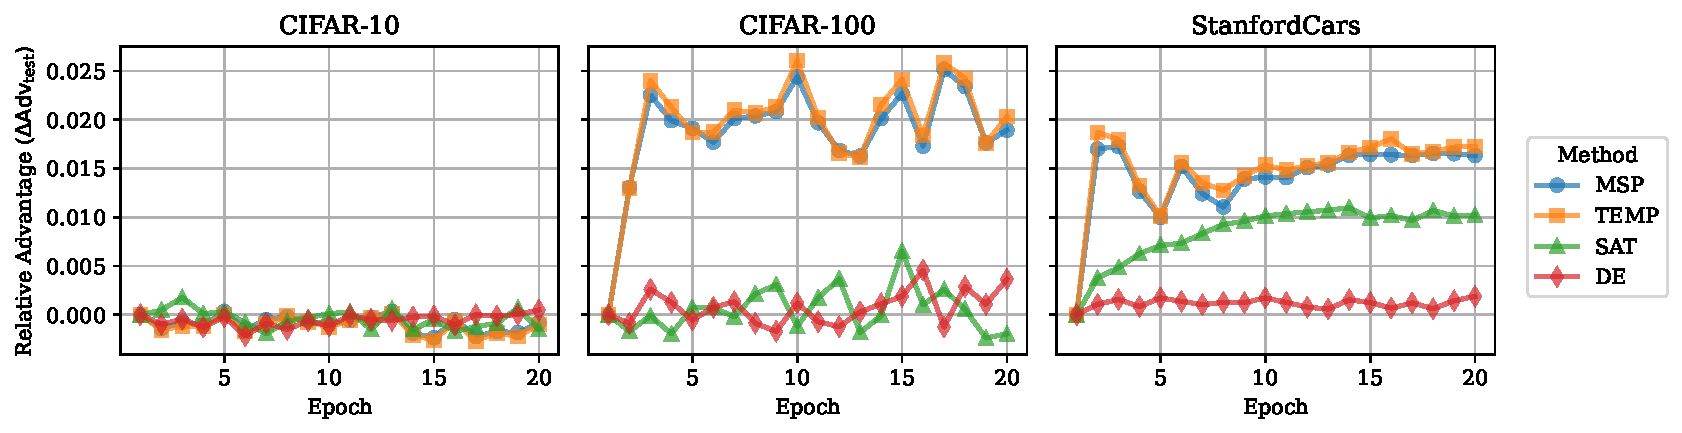
\includegraphics[width=1\linewidth]{figs/sc_bounds/adv_te.pdf}
    \caption[Relative LP advantage over training epochs across datasets.]{\textbf{Relative LP advantage over training epochs across datasets}. For each method, we plot the shift in test-set advantage $\Delta\mathrm{Adv}_{\mathrm{test}}(t)$ relative to epoch 1, indicating how much additional ranking signal the loss predictor learns over time. Larger values imply greater misalignment between the model’s confidence and correctness.}

    \label{fig:adv_te}
\end{figure}

\paragraph{Key Observations.}
On CIFAR-10 (left panel of Figure~\ref{fig:adv_te}), all methods stay close to zero $\Delta\mathrm{Adv}_{\mathrm{test}}$, indicating that the model's own confidence scores already capture most of the available ranking signal. On CIFAR-100 (middle panel), \texttt{MSP} and \texttt{TEMP} exhibit large positive shifts in LP advantage, suggesting that a dedicated loss predictor can substantially improve ranking—consistent with a larger gap from the oracle. By contrast, \texttt{SAT} and \texttt{DE} remain near zero, indicating that their confidence scores are already well aligned with correctness. On StanfordCars (right panel), the gap widens even further: both \texttt{MSP} and \texttt{TEMP} allow for significant gains via loss prediction, and even \texttt{SAT} leaves nontrivial room for improvement. Only \texttt{DE} consistently resists such gains, implying that deep ensembling is uniquely effective at preserving reliable ranking in high-variance domains.

\paragraph{Conclusion.}  
These results match our theory perfectly: whenever the LP head cannot improve on self-entropy, the selective classifier is effectively oracle‐optimal; whenever it can, the size of that advantage precisely quantifies the remaining ranking error and the gap from the ideal frontier.

\section{Additional Results}

\paragraph{Gap vs ECE} We provide additional comparisons on more datasets (CIFAR-10 and StanfordCars) on the relationship between the selective classification gap and the model's expected calibration error. See Tables~\ref{tab:cifar10_cal} and \ref{tab:stanfordcars_cal} for exact results. In general, our conclusions from Section~\ref{sec:calibration_ranking_exp} hold here as well: while temperature scaling (\temp) improves ECE over \msp, it does not reduce the selective classification gap—underscoring the limits of monotone calibration. In contrast, \sat and deep ensembles (\de) improve both ECE and gap by altering the ranking, confirming that only re-ranking methods yield meaningful gains in selective performance.

\begin{table}[h]
\fontsize{9}{10}\selectfont
\setlength{\tabcolsep}{5pt}
\caption{\textbf{Experiments on calibration across model classes on CIFAR-10}. Similar as Table~\ref{tab:cifar100_cal}}
\vspace{5pt}
\label{tab:cifar10_cal}
\centering
\begin{tabular}{lcccccccccccc}
\toprule
 & \multicolumn{4}{c}{CNN} & \multicolumn{4}{c}{ResNet-18} & \multicolumn{4}{c}{WideResNet-50} \\
\cmidrule(r){2-5} \cmidrule(r){6-9} \cmidrule(r){10-13}
 & \texttt{MSP} & \texttt{TEMP} & \texttt{SAT} & \texttt{DE} & \texttt{MSP} & \texttt{TEMP} & \texttt{SAT} & \texttt{DE} & \texttt{MSP} & \texttt{TEMP} & \texttt{SAT} & \texttt{DE} \\
\midrule
Gap & 0.024 & 0.023 & 0.019 & 0.016 & 0.004 & 0.004 & 0.003 & 0.002 & 0.003 & 0.003 & 0.002 & 0.002 \\
ECE & 0.075 & 0.025 & 0.035 & 0.010 & 0.025 & 0.014 & 0.016 & 0.007 & 0.027 & 0.022 & 0.019 & 0.010 \\
\bottomrule
\end{tabular}
\end{table}

\begin{table}[h]
\fontsize{9}{10}\selectfont
\setlength{\tabcolsep}{5pt}
\caption{\textbf{Experiments on calibration across model classes on StanfordCars}. Similar as Table~\ref{tab:cifar100_cal}}
\vspace{5pt}
\label{tab:stanfordcars_cal}
\centering
\begin{tabular}{lcccccccccccc}
\toprule
 & \multicolumn{4}{c}{CNN} & \multicolumn{4}{c}{ResNet-18} & \multicolumn{4}{c}{WideResNet-50} \\
\cmidrule(r){2-5} \cmidrule(r){6-9} \cmidrule(r){10-13}
 & \texttt{MSP} & \texttt{TEMP} & \texttt{SAT} & \texttt{DE} & \texttt{MSP} & \texttt{TEMP} & \texttt{SAT} & \texttt{DE} & \texttt{MSP} & \texttt{TEMP} & \texttt{SAT} & \texttt{DE} \\
\midrule
Gap & 0.176 & 0.177 & 0.166 & 0.159 & 0.030 & 0.029 & 0.26 & 0.022 & 0.026 & 0.026 & 0.23 & 0.020 \\
ECE & 0.110 & 0.025 & 0.058 & 0.025 & 0.040 & 0.027 & 0.037 & 0.025 & 0.017 & 0.017 & 0.015 & 0.015 \\
\bottomrule
\end{tabular}
\end{table}